%---------- Präambel ----------%

\documentclass[a4paper, numbers=noenddot, bibliography=totocnumbered, german,fontsize=11pt]{scrartcl} %Papierformat,Schriftgröße und Art des Dokumentes

\usepackage[utf8]{inputenc} %deutsche Umlaute
\usepackage[ngerman]{babel} %neue deutsche Rechtschreibung, sowie Silbentrennung
\usepackage[T1]{fontenc} %Westeuropäische Kodierung
\usepackage{lmodern} %modernes Schriftbild
%\usepackage{indentfirst} %einrücken des ersten Absatzes nach einer Überschrift

\usepackage{amsmath} %Mathematische Formeln
%\usepackage{ziffer} %Deutsches Komma und 1 000 er freistellen

\usepackage{pdfpages} %Einbinden von PDF-Seiten
\usepackage{graphicx} %Grafiken einfügen
\usepackage[per-mode=fraction, locale = DE]{siunitx} %Einheiten richtig darstellen

\usepackage{array} % Tabellenformate
\usepackage{tabulary} %dynamische Spaltenbreite
\usepackage{longtable} % Erzeugen mehrseitiger Tabellen
%\usepackage{ltxtable} % Kombination von Tabularx und Longtable
\usepackage{parnotes}
%\usepackage{footnote} %Fußnooten in Tabellen
%\makesavenoteenv{table}
%\makesavenoteenv{tabular} %Fußnoten in Tabellen
\usepackage{booktabs} %Dicke Linien in Tabellen
\usepackage{paralist} %Nummerierte Umgebung

\usepackage{float} %Grafik an genau diese stelle setzen (H)
\usepackage{wrapfig} %Grafik mit Textumfluss einfügen
%\usepackage{subfigure} %Grafiken nebeneinander darstellen

\usepackage{tocbasic} %Stil für Inhaltsverzeichnis
\usepackage[hidelinks,bookmarksopen,bookmarksopenlevel={1},bookmarksnumbered]{hyperref} %Verweise zwischen Nummern colorlinks für eingefärbte hyperlinks, frenchlinks für Kapitelchen.
%\usepackage{breakurl} %Verbeserter Zeilenumbruch bei urls (eigentlich nicht benötigt)
\usepackage{csquotes} %Zitate
%\usepackage[backref=true,backend=biber,style=numeric,sorting=none,hyperref=true]{biblatex} %Literaturverzeichnis mit Zahl und \cite verwenden
\usepackage[backref=true,backend=biber,style=numeric,sorting=none,hyperref=true,maxcitenames=2]{biblatex} %Literaturverzeichnis Harvard Style und \parencite verwenden
\DefineBibliographyStrings{ngerman}{ 
	andothers = {{et\,al\adddot}},             
}
%\usepackage[citation-order]{amsrefs} %Reihenfolge im Literaturzverzeichnis nach Aufruf

\usepackage{paracol}	%mehrere Spalten (Seitenaufteilung)
\usepackage{wasysym} %Durchmesserzeichen
%\usepackage[nofiller]{struktex} %Nassi-Shneidermann Diagramme
\usepackage{tikz} %Diagramme und Grafiken Zeichnen
\usepackage{pgfplots, pgfplotstable} %Diagramme Zeichnen
%\usepackage{mathtools} %Für mittlere Temperaturwerte
\usepackage{eurosym} %Eurozeichen
\usepackage{makecell} %Für Zeilenumbrüche in Tabellen
\usepackage{romannum} %Für römische Zahlen \Romannum{1} --> Große römische Zahl 
\usepackage{multirow} %Gegenteil von multicolumn
\usepackage[abs]{overpic} %Über Bilder malen


%\KOMAoptions{DIV=calc} %Teilung für optimalen Satzspiegel (führt oft zu geringer Seitenbreite)

%---------- Erhöht Abstandsmaße z.B. in Tabellen ----------%

\renewcommand*{\arraystretch}{1.5} %höhere Zeilen in tabellen

%---------- Literaturverzeichnis----------%

\nocite{*}%lässt alle Literatureinträge erscheinen (auch ohne Zitat)
\addbibresource{07_literaturverzeichnis.bib}
\defbibheading{head}{\section{Literatur}}
%---------- Zählung von Überschriften bei Verwendung von Paracol ----------%

%\globalcounter{figure} %Paracol durchzählen global Figuren
%\globalcounter{table} %Paracol durchzählen global Tabellen
%\globalcounter{equation} %Paracol durchzählen global Formeln
%\globalcounter{diagramm} %Paracol durchzählen global Diagramme
%\globalcounter{section} %Paracol durchzählen global Überschriften
%\globalcounter{subsection} %Paracol durchzählen global Unterüberschriften

%---------- Beschriftung der Tabellen und Abbildungen ----------%

\renewcaptionname{ngerman}{\figurename}{Abb.} %Beschriftung der Abbildungen
\renewcaptionname{ngerman}{\tablename}{Tab.} % Beschriftung der Tabellen

%---------- Wichtigbox Fynn (Formelsammlung) ----------%

%\usepackage{framed}
%\newenvironment{wichtigbox}{%
%	\def\FrameCommand{
%%		\fboxsep=-12pt 
%		\fboxrule 0.5mm \fcolorbox{red}{white}}%
%	\MakeFramed {\advance\hsize-\textwidth\FrameRestore}}%
%{\endMakeFramed}

%---------- Konfiguration von Diagrammen und Grafiken ----------%

\usetikzlibrary{
plotmarks,
arrows.meta,
calc,
arrows,
patterns,
positioning
}
\usepgfplotslibrary{patchplots}
\usepackage{grffile} % Für Matlab GRafiken
\pgfplotsset{
	plot coordinates/math parser=false,
	/pgf/number format/.cd,
	use comma,% Komma als Dezimaltrenner
	1000 sep = {\,}
}

\newlength\figureheight
\newlength\figurewidth

\pgfplotsset{
	compat=newest,
	samples=200,
	clip=false,
	my axis style/.style={
%		axis on top,
		axis x line=bottom,
		axis y line=middle,
%		scale only axis,
		legend pos= north east,
		axis line style={-{Latex[length=3mm]}},
		legend style={font=\normalsize},
		label style={font=\normalsize},
		tick label style={font=\normalsize},
		xlabel style={
			at={(ticklabel* cs:1)},
			anchor=west,
			font=\normalsize,
		},
		ylabel style={
			at={(ticklabel* cs:1)},
			anchor=west,
			font=\normalsize,
		},
		xlabel=x,
		ylabel=y,
		height=0.5\textwidth,
		width=0.75\textwidth,
	},
}

%---------- Absatz Texteinzug verändern----------%

\setlength{\parindent}{0pt} %Keine Texteinzüge am Absatzanfang

%---------- Einheiten Darstellungs Konfiguration ----------%

\sisetup{
	list-final-separator = { \translate{and} },
	list-pair-separator  = { \translate{and} },
	range-phrase         = { \translate{to (numerical range)}},
	group-minimum-digits={4}, %trennt auch Zahlen 4 Einheiten
%	group-separator={\,}, %kann den Gruppenseperator ändern
}

%---------- Ersetzt den Malpunkt mit \cdot ----------%

\DeclareMathSymbol{*}{\mathbin}{symbols}{"01} % macht alle Malzeichen als Punkt

%---------- Kapitelabhängige Nummerierung ----------%

\numberwithin{table}{section} %stellt den Tabellen eine section vorran
\numberwithin{figure}{section} %stellt den Bildern eine section vorran
\numberwithin{equation}{section} %stellt den Formelbeschriftungen eine section vorran

%---------- Spaltentypen für Tabellen ----------%

\newcolumntype{R}[1]{>{\raggedleft\arraybackslash}p{#1}}
\newcolumntype{C}[1]{>{\centering\arraybackslash}p{#1}}

%---------- Neue Verzeichnisstypen ----------%
\DeclareTOCStyleEntry[linefill=\hfill]{default}{subsection} %Subsections ohne Punktlinien

% Formelverzeichnis
%\DeclareNewTOC[
%type=equation,
%counterwithin=caption,
%name=Formel,
%listname={Formelverzeichnis},
%tocentryentryformat:=table,
%tocentrynumwidth:=table,%2.3em,% like figures and tables
%tocentryindent:=table,%1.5em,% like figures and tables
%]{loe}

% Diagrammverzeichnis
\DeclareNewTOC[
float,
floatpos = htp,                         % voreingestellte Gleitparameter
owner=float,
counterwithin=section,
type=diagramm,
name=Diagramm, % Name in Beschriftungen
listname={Diagrammverzeichnis},
tocentryentryformat:=table,
tocentrynumwidth:=table,%2.3em,% like figures and tables
tocentryindent:=table,%1.5em,% like figures and tables
]{lod}

% Anhangsverzeichnis
\DeclareNewTOC[%
owner=\jobname,
type=anhang,
listname={Anhangsverzeichnis},% Titel des Verzeichnisses
]{atoc}% Dateierweiterung (a=appendix, toc=table of contents)

\makeatletter
\newcommand*{\@currententry}{}
% Zwei amsmath-Anweisungen ändern:
\g@addto@macro\make@display@tag{\set@currententry}%
\def\tagform@#1{\maketag@@@{(\ignorespaces#1\unskip\@@italiccorr)}%
	\set@currententry}
\newcommand*{\set@currententry}{%
	\typeout{set current entry}%
	\ifx\@currententry\@empty\else
	\addcontentsline{loe}{table}{\protect\numberline{\@currentlabel}%
		\@currententry}%
	\global\let\@currententry\@empty
	\fi
}
% Neue Benutzeranweisung
\newcommand*{\equationentry}[1]{%
	\gdef\@currententry{#1}%
}
% Für Anhangsverzeichnis
\@addtoreset{section}{part}
\newcommand*{\useappendixtocs}{%
	\renewcommand*{\ext@toc}{atoc}%
}
\makeatother



%---------- Abmaße des Blattes mit Fuß- und Kopfzeile ----------%

\setlength{\headheight}{48.42pt}

\usepackage[headsepline]{scrlayer-scrpage} 	%Linien in Kopfzeile
\usepackage{scrlayer-scrpage}
\pagestyle{scrheadings}
\clearpairofpagestyles

\ihead{\textbf{Regenerative Energietechnik\\Kraftwerksreserven in Deutschland}\\\footnotesize{Moritz Deckert, Fynn Linnenbrügger}}
\ohead{
\includegraphics[height=15mm]{bilder/ostfalia.png}} %Logo Kopfzeile

%\ifoot{Linnenbrügger, Fynn} %Name im linken Feld
\cfoot{\today} %heutiges Datum \today
\ofoot{\pagemark} %aktuelle Seite

%---------- PDF-Eigenschaften ----------%

\hypersetup{pdftitle = {Die Energiewende -- Wo befinden sich Kraftwerksreserven in Deutschland?}
		pdfsubject  = {Die Energiewende -- Wo befinden sich Kraftwerksreserven in Deutschland?},
		pdfauthor   = {Moritz Deckert und Fynn Linnenbrügger}
	}

%---------- Titel, Autor, etc. für Deckblatt ----------%

\title{Die Energiewende -- Wo befinden sich Kraftwerksreserven in Deutschland?}
%\subtitle{Institut für energieoptimierte Systeme (EOS)}
%\author{Fynn Linnenbrügger}
%\date{\today} %heutiges Datum \today

%---------- Eigene Befehle ----------%

\newcommand*{\quelle}{\footnotesize Quelle: }
\newcommand*{\entspricht}{~\widehat{=}~}
\newcommand*{\uuline}[1]{\underline{\underline{#1}}}
\newcommand{\COO}{CO\textsubscript{2}} %CO2 schreiben
\newcommand{\Htwo}{H\textsubscript{2}} %H2 schreiben
\newcommand*{\stern}{\ast}
\DeclareSIUnit{\year}{\text{a}}
\DeclareSIUnit{\dH}{\text{°dH}}
\DeclareSIUnit{\litre}{\text{l}} % Kleinbuchstabe für Liter l
\DeclareSIUnit{\euro}{\text{\officialeuro}} %Eurozeichen im SI
\DeclareSIUnit{\L}{\text{L}} %Verbrennungsrechnung Luft
\DeclareSIUnit{\B}{\text{B}} %Verbrennungsrechnung Brennstoff
\DeclareSIUnit{\fA}{\text{fA}} %Verbrennungsrechnung feuchtes Abgas
\DeclareSIUnit{\tA}{\text{tA}} %Verbrennungsrechnung trockenes Abgas
\DeclareSIUnit{\Ntwo}{N_2} %Verbrennungsrechnung trockenes Abgas
\DeclareSIUnit{\Otwo}{O_2} %Verbrennungsrechnung trockenes Abgas
\DeclareSIUnit{\COtwo}{CO_2} %Verbrennungsrechnung trockenes Abgas
\DeclareSIUnit{\water}{H_2O} %Verbrennungsrechnung trockenes Abgas
\DeclareSIUnit{\Molpercent}{\text{Mol-\%}} %Verbrennungsrechnung trockenes Abgas
\DeclareSIUnit{\kW}{\text{kW}} %Kilowatt
\DeclareSIUnit{\qm}{\text{m^2}} %Quadratmeter
\DeclareSIUnit{\km}{\text{m^3}} %Kubikmeter
\DeclareSIUnit{\sonden}{\text{Sonden}} %Kubikmeter

%---------- Beginn der Arbeit ----------%

\begin{document}
\pagenumbering{arabic}
\setcounter{page}{0}	

\begin{center}
	\thispagestyle{empty}
	\tikz[remember picture,overlay] 
	\node[anchor=north east,inner sep=0pt]
	at([shift={(-.5,-.5)}]current page.north east){
\includegraphics[height=20mm]{bilder/ostfalia.png}}; 
	\vspace*{1cm}
	\centering
	\Large Fakultät Versorgungstechnik \\
	\textbf{\huge Hausarbeit} \\
	\vspace*{1cm}
	\Large im Modul Regenerative Energietechnik \\
	\vspace*{1cm}
	\Large zum Thema \\
	\vspace*{1cm}
	\huge{\textsf{\textbf{Die Energiewende -- Wo befinden sich Kraftwerksreserven in Deutschland?}}}
\end{center}

%\maketitle
\vspace*{1cm}
\large
\begin{center}
	\begin{tabular}{ll}
		vorgelegt von: & Moritz Deckert, 70455296 \vspace{2mm}\\	
		& Fynn Linnenbrügger, 70468167 \vspace{2mm}\\	
		Studiengang: & Energie- und Gebäudetechnik \vspace{2mm}\\
		& \\
		& \\	
		Prüfer:&Prof. Dr.-Ing. Oliver Büchel \vspace{2mm}\\	
		& Prof. Dr. Matthias Puchta \vspace{2mm}\\	
		& \\
		& \\
		Abgabedatum:& XY.01.2023
	\end{tabular}
\end{center}
%\begin{center}
%	Hiermit erklären wir, dass wir das Gasprojekt eigenständig\\
%	und nur mit den erlaubten Hilfsmitteln erstellt haben!
%	\vspace{8mm}\\
%	------------------------------------------------------\\
%	Hielscher, Jonas \vspace{8mm}\\
%	------------------------------------------------------\\
%	Linnenbrügger, Fynn \vspace{8mm}\\
%	------------------------------------------------------\\
%	Schröder, Caspar
%\end{center}

\include{01_Eidstaatliche_Erklärung.tex}
%\usetocstyle{normaltoc}
\pdfbookmark[1]{\contentsname}{normaltoc}
\tableofcontents
\clearpage
\listoffigures
%\clearpage
\listoftables
%\clearpage
%\listofdiagramms
\clearpage
\section*{Abkürzungsverzeichnis}
%	\textbf{Lateinische Buchstaben} \\ \\
%	\begin{tabulary}{\textwidth}{LLL}
%		\textbf{Symbol}&\textbf{Einheit}&\textbf{Bezeichnung}\\
%		$A_\mathrm{N}$&\si{\square\meter}&Energiebezugsfläche\\
%		%
%		$g$&\si{\meter\per\square\second}&Fallbeschleunigung\\
%		%
%	\end{tabulary} \clearpage
%
%	\textbf{Griechische Buchstaben} \\ \\
%	\begin{tabulary}{\textwidth}{LLL}
%		\textbf{Symbol}&\textbf{Einheit}&\textbf{Bezeichnung}\\
%		%
%		$\Phi_\mathrm{HL}$&\si{\kilo\watt}&Gesamtheizlast\\
%		%
%		$\Phi_\mathrm{HL,build}'$&\si{\watt\per\metre\squared}&Spezifische Gebäudeheizlast\\
%		%
%	\end{tabulary} \clearpage
%	
%	\textbf{Indizes und Abkürzungen} \\ \\
	\begin{tabulary}{\textwidth}{lL}
%		\textbf{Index}&\textbf{Bedeutung/ Anwendung}\\
		%
		ÜNB & Übertragungsnetzbetreiber \\
		%
		VNB & Verteilnetzbetreiber \\
		%
		EOM & Energy-Only-Market \\
		%
		BNetzA & Bundesnetzagentur \\
		%
		PRL & Primärregelreserve \\
		%
		ENTSO-E & European Network of Transmission System Operators for Electricity \\
		%
		SRL & Sekundärregelreserve \\
		%
		NRV & Netzregelverbund \\
		%
		MRL & Minutenreserve \\
		%
		EnWG & Energiewirtschaftsgesetz \\
		%
		BMWK & Bundesministerium für Wirtschaft und Klimaschutz		
	\end{tabulary} \clearpage

	

%\clearpage
%\listofequations
\pagestyle{scrheadings}
%\cleardoublepage

\section{Einleitung}

	Kraftwerksreserven sind im deutschen Stromsektor ein weitgefächerter Bereich, welcher einer Erklärung unter verschiedenen Gesichtspunkten bedarf.
	Dieser Begriff vereint mehrere Mechanismen zum Ausgleich von Angebot und Nachfrage am Strommarkt und der zuverlässigen Beständigkeit der Versorgungssicherheit in Deutschland.
	Ziel der folgenden Projektarbeit im Seminarfach "`Regenerative Energietechnik "` ist es die einzelnen Reserven genauer zu beleuchten und anhand unterschiedlicher Einflüsse zu analysieren.
	Im ersten Teil wird der Begriff der Kraftwerksreserve genauer untersucht, da es unterschiedliche Arten von Reserven gibt, um verschiedene Aufgaben zu bewältigen.
	Darüber hinaus wird das Funktionsprinzip des Strommarkts dargestellt, um die Unterschiede zu verdeutlichen.
	Der zweite Teil beschäftigt sich mit der Analyse von Kraftwerksreserven unter gesetzlichen, logistischen sowie wirtschaftlichen Gesichtspunkten.
	Im Anschluss wird Bezug auf die Bedeutung des Atom- und Braunkohleausstiegs für die Kraftwerksreserven genommen.	
	Zuletzt werden positive und negative Auswirkungen durch den Ausbau der erneuerbaren Energien auf die Kraftwerksreserven beleuchtet. \\
	
	Das Thema Versorgungssicherheit rückt nicht zuletzt durch den anhaltenden
	Ukraine Konflikt in den Fokus der Öffentlichkeit.
	Die unregelmäßigen Gaslieferungen aus Russland stellen eine Bedrohung für die deutsche Infrastruktur und Wirtschaft dar.
	Die dadurch verursachte Gasknappheit lässt die Preise für Energie in Deutschland und im Euroraum stark ansteigen.
	Nach Gesetzesänderungen der Bundesregierung rücken z.B. ältere Kohlekraftwerke aus unterschiedlichen Reserven in den Strommarkt nach, um die Verstromung aus Gas zu reduzieren und den Erdgasmarkt und -preis zu entspannen.
	Außerdem setzt der Ausbau der erneuerbaren Energien und die damit einhergehende Volatilität der Stromerzeugung, die Stromnetze vor eine enorme Herausforderung. 
	An dieser Stelle werden weitere Kraftwerksreserven benötigt, um das Netz zu entlasten und regionale Unterschiede in der Erzeugung auszugleichen. 
	Des Weiteren benötigt die Sicherung der Netzfrequenz weitere Ressourcen, um einen Zusammenbruch zu verhindern. 
	Für die schnelle Regelbarkeit der Frequenz stehen vier unterschiedliche Arten von Regelleistungsreserven zur Verfügung. 
	Im Anschluss wird nun auf die beschriebenen Thematiken Bezug genommen und auf die daraus resultierenden Herausforderungen für die Übertragungsnetzbetreiber (ÜNB) und Verteilnetzbetreiber (VNB) eingegangen. 
	
	
	
	
	
	
	\clearpage
\section{Wie kann der Begriff Kraftwerksreserve definiert werden?}

	Da der Begriff Kraftwerksreserve nicht genau definiert ist, wird im Folgenden auf die unterschiedlichen Arten der Kraftwerksreserven eingegangen.
	Grundlage bildet der Strommarkt, welcher in Kapitel \ref{sect: Wie funktioniert der deutsche Strommarkt?} behandelt wird.
	Aufgrund der Folgen des Ukraine-Konflikts ist ebenfalls eine weitere Art der Reserve hinzugekommen.

	\subsection{Wie funktioniert der deutsche Strommarkt?} \label{sect: Wie funktioniert der deutsche Strommarkt?}
	
		In Deutschland gibt es einen Energy-Only-Market (EOM).
		Dies bedeutet, dass ausschließlich der tatsächlich produzierte Strom gehandelt wird.
		Anders wäre dies bei dem viel diskutierten Kapazitätsmarkt, indem auch vorgehaltene Leistungen für z.B. Dunkelflauten vergütet werden (haucap).
		Die Preisbildung folgt dem Prinzip der Merit-Order (s. Abb. \ref{Abb. Strompreisbildung Merit Order}).
		In der Merit-Order werden alle Stromproduzenten, welche zu gegebenen Zeitpunkt ihren Strom am Markt anbieten, nach ihren jeweiligen Grenzkosten aufsteigend aufgelistet.
		Der Stromerzeuger mit den geringsten Grenzkosten, darf als erstes einspeisen und nach ihm derjenige mit den nächst größeren Grenzkosten.
		Als Grenzkosten werden die Erzeugungskosten für die auf dem Markt genau angebotene Strommenge bezeichnet.
		Der Stromproduzent, welcher mit seiner angebotenen Strommenge Angebot und Nachfrage deckt, legt den zu vergütenden Strompreis für alle anderen Marktteilnehmer in der Merit-Order unter ihm fest.
		Dieses Kraftwerk heißt Grenzkostenkraftwerk.
		In Abbildung \ref{Abb. Strompreisbildung Merit Order} ist die Reihenfolge der Stromerzeugungsart und den typisch zu erwartenden Grenzkosten dargestellt. \\
		
		\begin{figure} [H]
			\centering
			\label{Abb. Strompreisbildung Merit Order}
			\includegraphics[page=82,trim=150 282 140 375, clip, width=0.85\textwidth]{./anhang/Doktorarbeit Reitsam.pdf}
			\caption{Strompreisbildung an der Börse nach dem Merit-Order-Prinzip \parencite{Doktorarbeit_Reitsam}}
		\end{figure}
		
		In der Merit-Order weist die Stromerzeugung aus erneuerbaren Energien Grenzkosten von nahezu Null auf.
		Die Folge des Ausbaus von erneuerbaren Energien ist, dass konventionelle Kraftwerke mit hohen Grenzkosten, vor allem Gas- und Ölkraftwerke, in der Reihenfolge nach rechts gerückt werden (Merit-Order-Effekt, s. Abb. \ref{Abb. Strompreisbildung Merit Order}).
		Das Verdrängen der Gas-,Öl- sowie Pumpspeicherkraftwerke führen zu einem sinkenden Strompreis an der Böse \parencite{Frauenhofer_PV_Bericht}.
		Dadurch sind diese Kraftwerke nur bei mangelndem Wind und mangelnder Sonneneinstrahlung an der Stromproduktion beteiligt.
		Für den Strompreis bedeutet dies teilweise erhebliche Schwankungen je nach aktueller Wetterlage und geringe bzw. unvorhersehbare Betriebsstunden der genannten Marktteilnehmer. 
		Damit werden die Anreize vor allem schnell regelbare Gaskraftwerke zu errichten und wirtschaftlich betreiben zu können deutlich eingedämmt, weil die Kraftwerksleistung ohne Vergütung vorgehalten wird \parencite{Frauenhofer_PV_Bericht}.
		Gegensätzlich dazu verlangt der Ausbau regenerativer Stromerzeuger einen Zuwachs schnell regelbarer Gaskraftwerke, um plötzlich auftretende Schwankungen auszugleichen \parencite{Doktorarbeit_Reitsam}. \\
		
		Die Forderung eines Kapazitätsmarkts, indem auch vorgehaltene Kraftwerksleistung bepreist wird, gewinnt dahingehend an Bedeutung.
		Den Karftwerksbetriebern fällt es zunehmend schwer ihre konventionellen Kraftwerke aufgrund der bereits erörterten fehlenden und unvorhersehbaren Betriebsstunden rentabel zu betreiben.
		Auch ohne weiteren Ausbau von erneuerbaren Energien wird bei Dunkelflauten gerade in den wenig sonnigen Wintermonaten Januar und Februar weiterhin Residuallast gebraucht.
		Konträr dazu wurde eine strategische Kraftwerksreserve aus Braunkohlekraftwerken aufgebaut \parencite{bbh_blog}.		
				
	\subsection{Kraftwerksreserven zur Netzfrequenzstabilisierung}
	
		\begin{wrapfigure}{r}{0.55\textwidth}
			\centering
			\includegraphics[page=92,trim=260 71 50 450, clip, width=0.4\textwidth]{./anhang/Elektrizitätswirtschaft.pdf}
			\caption{Regelzonen und Übertragungsnetzbetreiber in Deutschland \parencite{Elektrizitätswirtschaft}}
			\label{Abb. Regelzonen Deutschland}
		\end{wrapfigure}
	
		Die Kraftwerksreserven zur Netzfrequenzstabilisierung fallen unter den Begriff des Regelenergiemarkts.
		Aufgrund des liberalisierten Strommarkts besitzen die Übertragungsnetzbetreiber keine eigenen Kraftwerke, sodass für die Stabilisierung Verträge mit Energieversorgungsunternehmen (EVU) geschlossen werden müssen. \\
			
		Unter Regelenergie versteht man zum einen die Reservierung von Kraftwerksreserven bzw. -kapazitäten (Regelleistung) und zum anderen den Ausgleich von Regelzonenungleichgewichten (Regelarbeit) \parencite{Elektrizitätswirtschaft}.
		Da es im Stromnetz zu negativen und positiven Abweichungen der Frequenz kommen kann, wird zur Kompensation sowohl positive als auch negative Regelarbeit benötigt.
		Anders als bei der Regelleistung wird eine gelieferte Strommenge in \si{\mega\watt\hour} vergütet.
		Um Unterschiede zwischen Angebot und Nachfrage unter den vier deutschen Regelzonen zu decken, wird eine Reservierung von Kraftwerksreserven erforderlich (Regelzonen s. Abb. \ref{Abb. Regelzonen Deutschland}). 
		In diesem Fall erfolgt eine Bezahlung der Kraftwerke unabhängig von der gelieferten Strommenge und Einsatzzeit \parencite{Elektrizitätswirtschaft}. 
		Die Bezahlung ist als eine Art Entschädigung für das Vorhalten von Kraftwerkskapazitäten, gegebenenfalls nicht Abrufen und den damit verbundenen Fixkosten der Einsatzbereitschaft zu verstehen.   
		
		\begin{figure} [H]
			\centering
			\label{Abb. Beispielhafte Darstellung der Regelenergie in Abhängigkeit der Netzfrequenz}
			\includegraphics[page=115,trim=50 80 50 470, clip, width=\textwidth]{./anhang/Elektrizitätswirtschaft.pdf}
			\caption{Beispielhafte Darstellung der Regelarbeit in Abhängigkeit der Netzfrequenz \parencite{Elektrizitätswirtschaft}}
		\end{figure}
	
		Um die Frequenz von \SI{50}{\hertz} im deutschen und europäischen Stromnetz stabil zu halten, muss ständig Regelarbeit eingesetzt werden.
		Für das ständige Abrufen der Regelarbeit wird Regelleistung gebraucht.
		Für die Netzfrequenz gibt es eine zulässige Schwankungsbreite von $\pm\SI{10}{\milli\hertz}$ \parencite{Angerer_Krohns}.
		Erst ab Unterschreitung von \SI{49,99}{\hertz} bzw. Überschreitung von \SI{50,01}{\hertz} wird die Frequenz durch Einsatz von Regelenergie stabilisiert.
		Bei einer zu geringen Netzfrequenz ist zu wenig Strom im Netz aufgrund von zu großer Abnahme oder Produktionsausfällen seitens der Stromerzeuger.
		In diesem Zuge gibt es Marktteilnehmer, welche zusätzliche Reserven bzw. Kapazitäten anbieten oder Stromverbraucher, die ihren eigenen Verbrauch drosseln.
		Gegensätzlich dazu ist eine zu hohe Netzfrequenz auf zu viel Strom im Netz zurückzuführen. 
		In diesem Fall wiederum können Stromverbraucher diesen erhöhen oder Stromerzeuger ihre Kraftwerksleistung herunterfahren. 
		In Abbildung \ref{Abb. Beispielhafte Darstellung der Regelenergie in Abhängigkeit der Netzfrequenz} ist die Abhängigkeit der Regelarbeit von der Netzfrequenz dargestellt.
		Für die beschrieben Mechanismen gibt es im Wesentlichen drei Regelenergien, die Primär-, Sekundärregelenergie und die Minutenreserve.
		Die Abbildung \ref{Abb. Reaktionskette Regelenergien} zeigt Regelenergiearten in ihrer Einsatzreihenfolge und Reaktionsschnelligkeit zur Stabilisierung der Netzfrequenz. 
		
		\begin{figure} [H]
			\centering
			\label{Abb. Reaktionskette Regelenergien}
			\includegraphics[page=209,trim=40 465 40 205, clip, width=\textwidth]{./anhang/Monitoringbericht_Energie2021.pdf}
			\caption{Zeitliche Abfolge der Regelleistungsreserven zur Netzfrequenzstabilisierung \parencite{Elektrizitätswirtschaft}}
		\end{figure}
		
		\subsubsection{Primärregelreserve} \label{sect: Primärregelreserve}
		
			Der Eingriff durch die Primärregelreserve (PRL) erfolgt unmittelbar nach Über- sowie Unterschreitung des zulässigen Frequenzbereichs durch die Anbieter von Primärreserven.
			Die Bereitstellung erfolgt über das Gebiet der ENTSO-E ("`European Network of Transmission System Operators for Electricity"').
			Da es sich bei dem ENTSO-E um ein Synchrongebiet mit \SI{50}{\hertz} Netzfrequenz handelt, wird die Bereitstellung von Primärregelleistung unter allen Teilnehmern, gemessen am eingespeisten Strom, aufgeteilt.
			Die Mitglieder können der Abbildung \ref{Abb. Mitglieder ENTSO-E} entnommen werden.
			Die gesamte Kapazität aller Mitglieder beläuft sich auf $\pm\SI{3}{\giga\watt}$ und wird anhand des zeitgleichen Ausfalls der zwei größten Kraftwerksblöcke innerhalb des Verbundnetzes ermittelt.
			Am Ort des Anbieters wird die Netzfrequenz gemessen, um schnell und frequenzabhängig Strom einzuspeisen oder zu speichern. 
			Innerhalb von \SI{30}{\second} muss die komplette Regelleistung abrufbar sein und die vollständig angebotene Regelarbeit für \SI{15}{\minute} geliefert werden.
			Der Regelbereich befindet sich dabei innerhalb des Regelbands und außerhalb des Totbands (s. Abb. \ref{Abb. Regelung Primarregelleistung} next Kraftwerke).
			Ab einer Netzfrequenz von \SI{49,99}{\hertz} bzw. \SI{50,01}{\hertz} muss der Stromlieferant die Primärregelleistung hochfahren und bei einer Frequenz von \SI{49,8}{\hertz} bzw. \SI{50,2}{\hertz} \SI{100}{\percent} seiner angebotenen Leistung abrufen bzw. liefern können. 
			
			\begin{figure}[H]
				\centering
				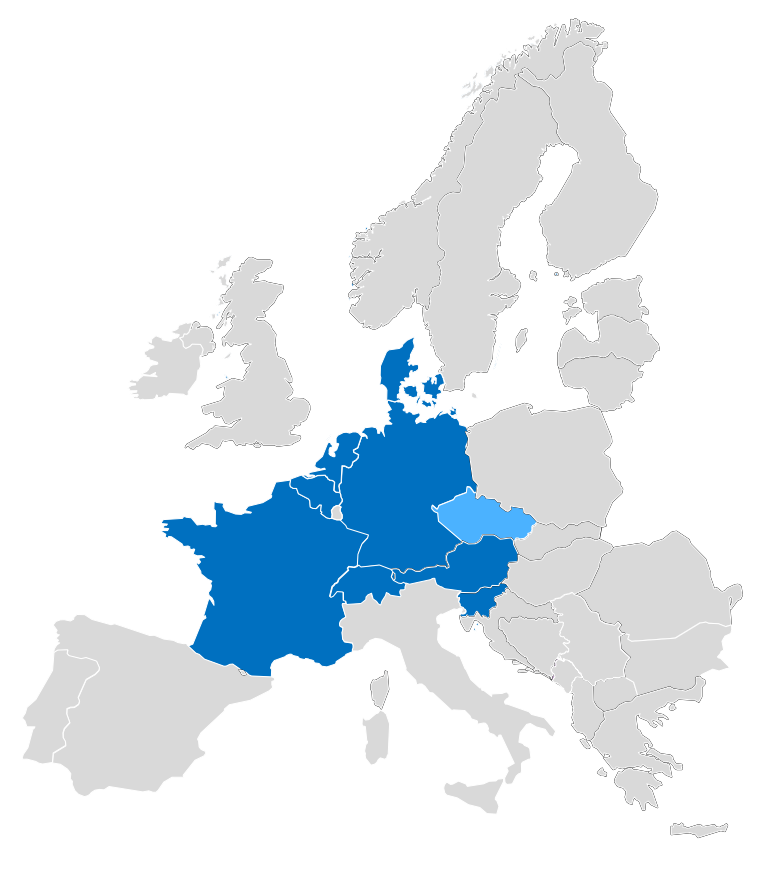
\includegraphics[page=1,trim=70 70 70 120, clip, width=0.6\textwidth]{./anhang/frc-map.png}
				\caption{Mitglieder der ENTSO-E für PRL\parencite{ENTSO-E_PRL}}
				\label{Abb. Mitglieder ENTSO-E}
			\end{figure}
			
			Die Ausschreibung von Primärregelleistung erfolgt täglich für einen Erbringungszeitraum vom Folgetag 0:00 Uhr bis 24:00 Uhr.
			Angebotsabgabe erfolgt am Vortag bis 8:00 Uhr  \parencite{regelleistungnet_PRL_Ausschreibung}.
			Die Auktion erfolgt online über die Internetseite regelleistung.net \parencite{regelleistungnet_PRL}.
			Zuschlag bekommen diejenigen Anbieter, welche für den ÜNB am wirtschaftlichsten sind.
			Der Anbieter, welcher Angebot und Nachfrage deckt, legt den Leistungspreis für alle anderen Zuschläger fest ("`Marginal Pricing"').
			In Tabelle \ref{Tab. Merkmale der Primärregellung} sind die wichtigsten Eckpunkte der Primärregeleistung dargestellt.		
		
			\begin{table}[H]
				\centering
				\caption{Merkmale der Primärregelleistung \cite{Regelleistung_NextKraftwerke}}
				\label{Tab. Merkmale der Primärregellung}
				\begin{tabular}{ll}
					\hline
					Regelenergieart & Primärregelleistung  \\ \hline
					Bereitstellung durch & ENTSO-E  \\
					Aktivierung & \makecell[l]{Frequenzgesteuert: \\ Eigenständige Messung/Eingriff vor \\ Ort durch Anbieter der PRL} \\
					Volle Leistung & Innerhalb von 30 Sekunden \\
					\makecell[l]{Abzudeckender Zeitraum \\ nach Störungsfall} & \num{0} bis \num{15} Minuten  \\
					Vergütung & Leistungspreis  \\
					Mindestangebots-größe & Ab $\pm\SI{1}{\mega\watt}$ (symmetrisch) \\
					Tägliche Produkte & \makecell[l]{Positiv und negativ: \\ \num{6} Zeitintervalle über \num{4} Stunden} \\ \hline
				\end{tabular}
			\end{table}
		
		\subsubsection{Sekundärregelreserve}		
			
			Bei länger anhaltender Frequenzabweichung wird die Sekundärregelreserve (SRL) hinzu geschaltet, um die Frequenz durch sowohl positive als auch negative Regelleistung wieder zu stabilisieren.
			Sie wird durch den innerhalb der Regelzone aktiven Übertragungsnetzbetreiber per Signal angefordert und durch die an der Auktion teilgenommenen Anbieter von SRL abgerufen. 
			Die SRL wird nach \num{30} Sekunden hinzu geschaltet und muss nach fünf Minuten volle Regelarbeit liefern können. 
			Für den täglichen Abruf der Reserve gibt es sechs Zeitscheiben mit je vier Stunden.
			Aufgrund dessen, dass die Sekundärregelleistungsanbieter ihre Anlagen im Verbund nicht auf einige \si{\mega\watt} modulieren können, besteht kontinuierlicher Bedarf an Sekundärregelleistung.
			Da jeder ÜNB in seiner Regelzone SRL zu- und abschalten kann, besteht eine Austauschpflicht unter den vier ÜNB.
			Der Grund ist, dass auf diese Weise ineffizientes gegeneinander regeln vermieden werden soll \parencite{SRL_NextKraftwerke}. \\
			
			Die Mindestangebotsgröße beträgt \SI{5}{\mega\watt} und nach einer Änderung des Beschlusses "`zur Festlegung von Ausschreibungsbedingungen und Veröffentlichungspflichten für Sekundärregelung"' der BNetzA können auch Angebote in Höhe von \SI{1}{\mega\watt} bis \SI{4}{\mega\watt} eingereicht werden.
			Diese Änderung ist an die Maßgabe geknüpft, dass die Anbieter ausschließlich ein Angebot je Produktscheibe für positive oder negative Regelleistung abgeben dürfen \parencite{Beschluss_SRL}.
			Die Reduzierung erleichtert den Eintritt für kleinere Anbieter oder jene, welche mehrere Anlagen poolen und meist zu virtuellen Kraftwerken verbinden. \\
			
			Die Ausschreibungen für die Sekundärregelreserven finden täglich statt. 
			Bis zum Vortag um 9:00 Uhr muss das Angebot für den Folgetag abgegeben werden.
			Es wird aufgeteilt nach dem Leistungs- und Arbeitspreis vergütet.
			Dies bedeutet, dass jeder Anbieter einen Festpreis für die Vorhaltung der angebotenen Leistung abgibt, egal ob diese abgerufen wird (Handel auf dem Regelleistungsmarkt).
			Der abgegebene Arbeitspreis wird auf dem Regelarbeitsmarkt gehandelt und gibt an wie hoch die Vergütung je erbrachter \si{\mega\watt\hour} ist.
			Die Art der Vergabe erfolgt nach der aufgestellten Merit-Order-Liste allerdings in einem Pay-as-Bid Verfahren(s. Kapitel \ref{sect: Primärregelreserve}).
			Es wird lediglich der angebotene Preis vergütet und nicht wie bei der PRL durch das "`Marginal Pricing"'.
			Tabelle \ref{Tab. Merkmale der Sekundärregelreserve} zeigt nochmals die wichtigsten Eckdaten der Sekundärregelreserve.
			
			\begin{table}[H]
				\centering
				\caption{Merkmale der Sekundärregelreserve \cite{Regelleistung_NextKraftwerke}}
				\label{Tab. Merkmale der Sekundärregelreserve}
				\begin{tabular}{ll}
					\hline
					Regelenergieart &  Sekundärregelreserve  \\ \hline
					Bereitstellung durch  & ÜNB  \\
					Aktivierung & \makecell[l]{Durch verantwortlichen ÜNB \\ - manuelle Anforderung durch ÜNB} \\
					Volle Leistung & Innerhalb von 5 Minuten \\
					\makecell[l]{Abzudeckender Zeitraum \\ nach Störungsfall} & ab 30 Sekunden bis 15 Minuten \\
					Vergütung &  Leistungs- und Arbeitspreis \\
					Mindestangebots-größe & \SI{5}{\mega\watt} positiv oder negativ\parnote{Eine Angebotshöhe von \SI{1}{\mega\watt} bis \SI{4}{\mega\watt} ist zulässig, sobald ein Anbieter von Minutenreserve nur ein einziges Angebot je Zeitscheibe für positive oder negative MRL in der jeweiligen Regelzone abgibt.}\\
					Tägliche Produkte & \makecell[l]{Positiv und negativ: \\ \num{6} Zeitintervalle über \num{4} Stunden} \\ \hline
				\end{tabular}
				\parbox{0.7\textwidth}{\parnotes}
			\end{table}
	
		\subsubsection{Minutenreserve}
		
			Die Minutenreserve ist die dritte aktive Maßnahme zur Stabilisierung der Netzfrequenz. 
			Falls die Sekundärregelreserve es nicht innerhalb von \num{15} Minuten schafft die Frequenz entsprechend zu stabilisieren, muss die Minutenreserve innerhalb von weiteren \num{15} Minuten auf volle Leistung hoch fahrbar sein.
			Die Mindestangebotsgröße beträgt wie bei der Sekundärregelreserve \SI{5}{\mega\watt} und unter der bereits erläuterten Maßnahme können auch Angebote in Höhe von mindestens \SI{1}{\mega\watt} abgegeben werden.
			Unter diesem Aspekt ist das Pooling von Anlagenleistung möglich und erleichtert somit den Einstieg kleinerer Anbieter.
			Es wird sich ebenfalls auf sechs Zeitscheiben über je vier Stunden beworben. \\
			
			Vergütet wird wie bei der Sekundärreserve aufgeteilt nach dem Leistungs- und Arbeitspreis.
			Das einreichen von Angeboten und die darauffolgende Vergabe verläuft exakt gleich der Vergabe von Sekundärregelleistungsreserve.
			Die Angebotsabgabefrist verschiebt sich lediglich um eine Stunde nach hinten auf 10:00 Uhr.
	
			\begin{table}[H]
				\centering
				\caption{Merkmale der Minutenreserve \cite{Regelleistung_NextKraftwerke}}
				\label{Tab. Merkmale der Minutenreserve}
				\begin{tabular}{ll}
					\hline
					Regelenergieart  & Minutenreserve \\ \hline
					Bereitstellung durch & ÜNB \\
					Aktivierung & \makecell[l]{Durch verantwortlichen ÜNB \\ - löst automatisch PRL ab}\\
					Volle Leistung & Innerhalb von 15 Minuten \\
					\makecell[l]{Abzudeckender Zeitraum \\ nach Störungsfall} & ab 15 Minuten bis 60 Minuten \\
					Vergütung & Leistungs- und Arbeitspreis \\
					Mindestangebots-größe & \SI{5}{\mega\watt} positiv oder negativ\parnote{Eine Angebotshöhe von \SI{1}{\mega\watt} bis \SI{4}{\mega\watt} ist zulässig, sobald ein Anbieter von Minutenreserve nur ein einziges Angebot je Zeitscheibe für positive oder negative MRL in der jeweiligen Regelzone abgibt.} \\
					Tägliche Produkte & \makecell[l]{Positiv und negativ: \\ \num{6} Zeitintervalle über \num{4} Stunden} \\ \hline
				\end{tabular}
				\parbox{0.7\textwidth}{\parnotes}
			\end{table}
		
		\subsubsection{Primärenergieträger und Einsatzzeiten}
			
			Aus Tabelle \ref{Tab. Übersicht der Präqualifizierten Leistung je PrimärenergieträgerKategorie in Deutschland} können die Präqualifizierten Leistungen je Primärenergieträger in Deutschland entnommen werden.
			Auffällig ist der hohe Anteil an Wasserkraft und Erdgas mit \SI{64,3}{\percent} und \SI{15,1}{\percent} an der Sekundärreserve bzw. \SI{42,3}{\percent} und \SI{21,1}{\percent} an der Minutenreserve.
			In der Minutenreserve ist ebenfalls ein großer Anteil an konventionellen Braun- und Steinkohlekraftwerken in Höhe von \SI{21,5}{\percent}.
			Die vorgehaltene Leistung verhält sich aufsteigend von der Primär- bis zur Minutenreserve.
			Des Weiteren ist gut zu erkennen, dass Windkraft, Batteriespeicher und Demand-Side-Management Systeme kaum eine Rolle für die Bereitstellung von Kraftwerksreserve zur Netzfrequenzstabilisierung spielen. \\
			
			Um die Diversität der Teilnehmer am Regelleistungsmarkt zu analysieren, kann die von den ÜNB veröffentliche Liste genutzt werden \cite{regelleistungnet_PRL_Ausschreibung}.
			Auf der Liste sind insgesamt \num{53} Unternehmen aufgeführt, welche am Regelleistungsmarkt ihre Kapazitäten zur Verfügung stellen.
			Ausschließlich Unternehmen, welche die Präqualifikationskriterien des in der Regelzone verantwortlichen ÜNB erfüllen, dürfen am Regelleitungsmarkt teilnehmen.
			Die Mehrzahl der aufgelisteten Marktteilnehmer sind Energieversorgungsunternehmen oder solche, die sich auf Energie- und Systemdienstleistungen konzentrieren.
			Lediglich acht Unternehmen sind aus der Industrie wie der Ludwigshafener Chemiekonzern BASF oder Trimet Aluminium SE.
			Die aufgelisteten Industriekonzerne bieten in erster Linie Sekundär- und Minutenreserve an.
			Die wenigen Industrieunternehmen, die Primärreserven vorhalten, haben sich auf Batteriespeicher spezialisiert und können somit schnelle bzw. dynamische Reserven zur Verfügung stellen.
			Nach Stand vom 28.01.2022 haben 30 Unternehmen Primärregelleistung, jeweils 34 Sekundärregelleistung und Minutenreserve angeboten. 
						
			\begin{table}[H]
				\renewcommand*{\arraystretch}{1.3} %höhere Zeilen in tabellen
				\centering
				\caption{Übersicht der Präqualifizierten Leistung (in \si{\giga\watt}) je Primärenergieträger/Kategorie in Deutschland, Stand: 01.01.2022 \cite{regelleistungnet_PRL_Ausschreibung}}
				\label{Tab. Übersicht der Präqualifizierten Leistung je PrimärenergieträgerKategorie in Deutschland}
				\begin{tabular}{lrrrrr}
					\hline
					Technologie & FCR  & aFRR$+$ & aFRR$-$& mFRR$+$ & mFRR$-$ \\ \hline
					Kernenergie & 0,22 & 0,18 & 0,19 & 1,27 & 1,27 \\
					Braunkohle & 0,56 & 1,20 & 1,21 & 4,16 & 4,20 \\
					Steinkohle & 0,48 & 1,05 & 1,07 & 2,98 & 2,88 \\
					Erdgas & 0,35 & 3,53 & 3,57 & 7,10 & 6,94 \\
					Öl & - & 0,26 & 0,03 & 1,28 & 0,09 \\
					Biogas/-masse & 0,04 & 1,82 & 2,29 & 2,27 & 2,75 \\
					Wasser & 4,79 & 15,10 & 15,15 & 13,99 & 14,01 \\
					Batteriespeicher & 0,48 & 0,08 & 0,06 & - & - \\
					Nachfrage/DSM & 0,02 & 0,12 & 0,07 & 0,20 & 0,14 \\
					Windkraft & - & - & 0,03 & - & 0,22 \\
					Sonstige & - & 0,01 & 0,01 & 0,11 & 0,30 \\ \hline
					Summe & 6,94 & 23,35 & 23,68 & 33,36 & 32,80
				\end{tabular}
				\renewcommand*{\arraystretch}{1.5} %höhere Zeilen in tabellen
			\end{table}
			
			Aus dem Mo­ni­to­ring­be­rich­t der BNetzA geht hervor, dass die Primärregelreserven ständig und unmittelbar abgerufen werden. 
			Es findet also eine ständige Korrektur der Netzfrequenz statt.
			Ähnlich verhält es sich bei der Sekundärregelleistung. 
			In nahezu jeder der jährlichen \num{35040} Viertelstunden kommt die Sekundärregelreserve zum Einsatz.
			Im Hinblick auf die Minutenreserve kann ein deutlicher Rückgang zum Vorjahr verzeichnet werden (2019: 8313 und 2020: 3230 \cite{Monitoringbericht_BNetzA}.
			Auffallend ist ebenso, dass die positive MRL deutlich häufiger als die negative abgerufen wird (s. Tab. \ref{Tab. Abrufen von Minutenreserve}).
			Dies lag unter anderem am von Oktober 2018 bis Juli 2019 angewandten Mischpreisverfahren.
			Durch ansteigen vorrangig der Leistungspreise für die Bereitstellung von Regelleistung , sind die Arbeitspreise gesunken, welche nur bei einem Abruf von Regelenergie gezahlt werden.
			Demnach ergaben sich wenig Anreize für Bilanzkreisverantwortliche ihre Netzprognosen sorgfältig abzugeben, da die bei Ungleichgewichten gezahlten Arbeitspreise zur aktiven Regulierung der Netzfrequenz sehr billig waren.
			Somit war es wirtschaftlicher Angebot und Nachfrage über Aktivierung von Regelreserven als durch sorgfältige Verbrauchsprognosen zu regulieren \cite{Monitoringbericht_BNetzA}.
						
			\begin{table}[H]
				\centering
				\caption{Einsatzhäufigkeit von positiver und negativer Minutenreserve \cite{Monitoringbericht_BNetzA}}
				\label{Tab. Abrufen von Minutenreserve}
				\begin{tabular}{lrr}
					\hline
					Einsatzhäufigkeit & 2019 & 2020 \\ \hline
					MRL positiv & 5271 & 2256 \\
					MRL negativ & 3042 & 974 \\ \hline
				\end{tabular}
			\end{table}
			
								
		\subsubsection{Momentanreserve}
		
			Eine weitere Möglichkeit zur Frequenzstabilisierung stellt die Momentanreserve dar.
			Sie ist im Sinne der klassischen Regelleistungen wie PRL, SRL und MRL keine Systemdienstleistung, da die ÜNB keinen direkten Einfluss auf diese haben.
			Momentanreserven sind rotierende Schwungmassen aus z.B. Generatoren, welche intrinsisch auf die Netzfrequenz wirken.
			Die Momentanreserve greift noch vor der Primärregelleistung ein und wirkt dadurch unmittelbar auf das Netz ohne das sie gezielt ab- oder zugeschaltet wird.
			Generatoren, die direkt an das deutsche Stromnetz angeschlossen sind, sind auf eine Netzfrequenz von \SI{50}{\hertz} eingestellt.
			Bei Frequenzabfall oder -anstieg drehen sich die Schwungmassen der Generatoren langsamer oder schneller und wirken der Frequenzabweichung dämpfend entgegen \cite{Gawlik}.		
			Um die Frequenz innerhalb des Regelbands zu halten und Ausreißern entgegenzuwirken, nutzen diese die gespeicherte kinetische, magentische oder elektrische Energie \cite{Energiespeicher}.
			Bei Ausbau der erneuerbaren Stromerzeuger allem voran Wind- und Sonnenenergie sind unmittelbar abrufbare Momentanreserven für die Aufrechterhaltung der Stromversorgung von zentraler Rolle.
			Die dauerhaft vorzuhaltene Momentanreserve bemisst sich an einem maximalen Leistungssprung bzw. Lastabfall von \SI{3}{\giga\watt} \cite{Bericht_Momentanreserve}. \\
			
			Aufgrund des direkten Zusammenhangs zwischen dem mechanischen Moments und der elektrischen Leistung ändert sich die Rotationsgeschwindigkeit in Abhängigkeit der Netzfrequenz.
			Die rotierende Schwungmasse wirkt aufgrund ihrer Massenträgheit durch Aus- und Einspeichern von Rotationsenergie einer Änderung der Rotatationsgeschwindigkeit entgegen \cite{Bericht_Momentanreserve}.
			
			\begin{align}
				P_\mathrm{el}&=M*\num{2}*\pi*f \\
				M&=J*w \\
				E_\mathrm{rot}&=\frac{\num{1}}{\num{2}}*J*\omega
			\end{align}
		
	\subsection{Kraftwerksreserven zur Reserveleistungsvorhaltung}
	
		Abbildung \ref{Abb. Reserven Deutschland} zeigt die deutschlandweite Verteilung von Netz-, Kapazitätsreserven und den Braunkohlekraftwerken der Sicherheitsbereitschaft.
		Die drei Arten der Reserveleistungsvorhaltung sind im Energiewirtschaftsgesetz gesetzlich verankert und gegenwärtige Rahmenbedingungen klar definiert.
		Anhand der Karte wird verdeutlicht, dass die Netzreserve vor allem in Süddeutschland präsent ist (orange Kennzeichnung).
		Die Gründe für die überaus starke regionale Konzentration im Süden werden in Kapitel \ref{sect: Netzreserve} eruiert.
		Die rot gekennzeichneten Kapazitätsreserven sind hauptsächlich im Norden Deutschlands zu finden.
		Die drei verbliebenen Braunkohlekraftwerke aus der Sicherheitsbereitschaft sind mit blauen Punkten gekennzeichnet.
		
		\begin{figure} [H]
			\centering
			\begin{overpic}[width=0.5\textwidth]{./anhang/Karte Kraftwerke.pdf}%
				\put(200,45){\small Netzreserve}%
				\put(200,35){\small Kapazitätsreserve}%
				\put(200,25){\small Sicherheitsbereitschaft}%
			\end{overpic}
			\caption{Netz-,Kapazitätsreserven und Sicherheitsbereitschaft in Deutschland, Quelle: Eigene Darstellung}
			\label{Abb. Reserven Deutschland}
		\end{figure}
	
		\subsubsection{Netzreserve} \label{sect: Netzreserve}
		
			Die Netzreserve stellt den ÜNB zusätzliche Kraftwerkskapazitäten für den Redispatch zur Verfügung, um zwischenzeitlich auftretende Lastspitzen abzufedern.
			Redispatch bezeichnet dabei die Maßnahme einen netzseitigen Engpass auszugleichen.
			In den meisten Fällen wird diese Maßnahme mit dem Nord-Süd-Gefälle des Stromnetzes in Verbindung gebracht.
			Besonders massiv zeigt sich dieses Problem im Winterhalbjahr, da der allgemeine Strombedarf größer ist.
			Die Windparks im Norden des Landes produzieren viel Strom, welcher unter anderem aufgrund des mangelnden Netzausbaus nicht von Nord nach Süd transportiert werden kann.
			Um diesen Engpässen entgegenzuwirken und ein Gleichgewicht herzustellen, werden im Norden Kraftwerke heruntergefahren und im Süden mit der gleichen Leistung hochgefahren.
			So findet ein Ausgleich bzw. eine Entlastung über die Grenzen der Regelzonen hinweg statt.
		
		\subsubsection{Kapazitätsreserve}
		
		
		\subsubsection{Sicherheitsbereitschaft}
\section{Bewertung der Kraftwerksreserven zur Netzstabilisierung und Reserveleistungsvorhaltung}

Im vorherigen Kapitel wurden die verschiedene Reserven in Deutschland beleuchtet und definiert. Außerdem fand eine erste Bewertung der aktuellen Situation statt. Im folgenden sollen nun die technische und logistische Realisierbarkeit bzw. Nutzbarkeit der verschiedenen Reserven beleuchetet werden. Außerdem soll ein Ausblick auf zukünftige Entwicklungen, Möglichkeiten und Gefahren gegeben werden.

Dabei spielt auch der russische Überfall auf die Ukraine eine Rolle. Diese wird in einer Aufnahme der momentanen deutschen Strategie zur Versorgungssicherheit im Winter berücksichtigt.

	\subsection{Bewertung nach logistischen Gesichtspunkten}
	Die Erhebung der Daten im Punkt Logistik gestaltete sich als herausfordernd. Hier gab es das Problem, dass keine unabhängige Stelle die logistische Situation tatsächlich im Blick hat. Aussagen konnten nur von den Kraftwerksbetreibern selbst getätigt werden.
	
		\subsubsection{Logistischer Stand bei der Braunkohle (Arbeitstitel)}
		Braunkohlekraftwerke befinden sich in Deutschland ausschließlich in der Sicherheitsbereitschaft. Die zwei Betreiber sind die RWE Power AG mit den zwei Blöcken Niederaußem E und F in Bergheim und dem Block Neurath C in Grevenbroich im Rheinischen Braunkohlerevier und die Lausitzer Energie und Kraftwerke AG, im folgenden LEAG, mit den zwei Blöcken Jänschwalde E und F in Teichland im Lausitzitzer Braunkohlerevier. \\
		
		Die Blöcke des Kraftwerks Jänschwalde werden durch Tagebaue der LEAG in Jänschwalde, Welzow-Süd, Nochten und Reichwalde versorgt. Der Einzugsradius beträgt (hier km Radius). Der Transport wird auf der Schiene durch einen firmeneigenen Eisenbahnbetrieb realisiert. Der Abbau des Tagebaus Jänschwalde stoppt voraussichtlich im Jahr 2023. Dann ist der Tagebau erschöpft. Die Versorgung wird dann von den übrigen drei Abbaustandorten übernommen.
		Da es sich beim Kraftwerk Jänschwalde um ein Großkraftwerk mit 6 Blöcken handelt gibt es kein Personalproblem. 
		(Hier noch etwas zum Wiedereinstieg in den Markt)\\
		
		Die in Sicherheitsbereitschaft befindlichen Blöcke Niederaußem E und F sowie Neurath C werden ebenfalls durch RWE-eigene Tagebaue versorgt. Hierbei handelt es sich um die Förderstätten Garzweiler, Hambach und Inden. Der Einzugsradius beträgt (km) für das Kraftwerk Neurath und (km) für das Kraftwerk Niederaußem. Der Transport erfolgt über eine Eisenbahngesellschaft der RWE. Auch bei diesen drei Blöcken handelt es sich um Teile von größeren Kraftwerkskomplexen. Daher stellt die Personalsituation kein Problem dar.
		
		\subsubsection{Logistischer Stand bei der Steinkohle}
		Die deutschen Steinkohlekraftwerke, welche nicht mehr aktiv am Markt teilnehmen und noch nicht endgültig stillgelegt sind, befinden sich in Deutschland in der Netzreserve. Diese ist durch das Kohleverstromungsbeendigungsgesetz, nachfolgen KVBG genannt, und Paragraph 13b des Energiewirtschaftsgesetzes, im weiteren Verlauf EnWG, rechtlich verankert. Bei den Betreibern handelt es sich um die EnBW Energie Baden-Würtemberg AG, die STEAG, Uniper Kraftwerke GmbH, Kraftwerk Mehrum GmbH und das Großkraftwerk Mannheim. \\
		
		Die logistische Situation war und ist angespannt. Niedrige Pegelstände von Rhein und Neckar, sowie der fehlende Gleisausbau in Deutschland erschwerten den Steinkohletransport deutlich. Die RAG Deutsche Steinkohle AG war der alleinige Betreiber deutscher Steinkohlebergwerke. Diese stellte den Abbau 2018 komplett ein, da ein wirtschaftlicher Abbau nicht mehr möglich war(Quelle). Damit sind die Betreiber zu \SI{100}{\percent} auf Importe angewiesen.\\
		
		Die EnBW mit den Standorten Heizkraftwerk Altbach/Deizisau HKW 1, Heizkraftwerk Heilbronn HLB 5 und 6 sowie dem Kraftwerk Walheim mit den Blöcken 1 und 2 verstärkte ab Juli 2022 ihre Bemühungen zur Beschaffung, sowie der Erschließung von Flächen zur zusätzlichen Lagerung von Steinkohle.(Pressemeldung und Mail) Auch die Personalsituation ist angespannt, da diese langfristig mit der Premisse der Stillegung geplant wurde. Die fünf Blöcke, welche sich in Netzreserve befinden, werden jedoch aller Voraussicht nach nicht wieder am Markt teilnehmen. Diese können nach eigener Aussage der EnBW aus technischen Gründen nicht ununterbrochen zur Stromerzeugung eingesetzt werden. Grund hierfür ist das fortgeschrittene Alter der Anlagen.\\
		
		Der Stromerzeuger STEAG betreibt zwei Kraftwerke in Netzreserve, die Standorte Boxberg und Weiher 3 im Saarland. Die herausfordernde Lage der Kohleversorgung, auch mit hinblick auf den kommenden Winter, veranlasste das Wirtschaftsministerium des Saarlandes zu einem Logistik-Gipfel. Zu den Teilnehmenden gehörten unter Anderen der Staatssektretär des Bundesministeriums für Digitales und Verkehr, die STEAG selbst und die DB Cargo. Die Gespräche ergaben eine vorrangige Behandlung von Kohletransporten auf der Schiene gegenüber dem öffentlichen Personennahverkehr, im Falle von Versorgungsengpässen. Dies sichert die Belieferung der Kraftwerke mit Brennstoff. Zusätzlich tritt das Kraftwerk Boxberg zum 28.10.2022 wieder in den Markt ein. Das Schwesterkraftwerk Weiher 3 folgte am 31.10.2022. Ermöglicht wird dies durch das Ersatzkraftwerkbereithaltungsgesetz, kurz EKBG, welches eine Rückkehr in den Strommarkt bis Frühjahr 2024 gestattet.\\
		
		Hier Uniper, Mehrum und GKW Mannheim sobald Informationen vorhanden.
		
		\subsubsection{Logistischer Stand beim Gas}
		In Folge des russischen Überfalls auf die Ukraine sanken die deutschen Erdgasimporte aus Russland im September nach Stand 03.11.2022 auf null. Zum 03.05.2022 startete die Bundesnetzagentur eine Datenerhebung um den deutschen Gasverbrauch zu ermitteln. In einer Pressemitteilung vom 29.09.2022 wurde von einer notwendigen Einsparung in Höhe von \SI{20}{\percent} gesprochen um die Versorgungssicherheit auch von Erdgaskraftwerken im Winter zu gewährleisten, das Impulspapier von Acatech spricht sogar von 20 bis \SI{30}{\percent}.\\
		
		Deutsche Erdgaskraftwerke, welche nicht mehr im Betrieb sind, befinden sich sowohl in der Netz- als auch in der Kapazitätsreserve. Die Versorgung ist sehr stark von den Netzbetreibern abhängig und die Situation sehr schwer vorhersehbar. Deutschland verfügt zum 04.11.2022 über ein LNG-Terminal zum Import von verflüssigtem Erdgas in Lubmin. Ein weiteres soll im Winter in Betrieb gehen.
		Ein zusätzliches Problem bei der Versorgung besteht in der Ausrichtung der in Europa vorhandenen Gas-Infrastruktur. Dieses ist durch den Aufbau auf einen Gastransport von Ost nach West ausgerichtet. Der Großteil der europäischen LNG-Terminals befindet sich in Westeuropa. Damit ist eine Umkehrung des Gasflusses notwendig. Dieser sogenannte Reverse-Flow wird ermöglicht, indem die Verdichterstationen umgebaut werden. Danach ist ein Gastransport in beide Richtungen bei voller Kapazität möglich.(acatec Impuls)\\
		
		Ein eventuelles Verbot der Verstromung von Gas ist im Notfallplan Gas beschrieben. Dieser ist in drei Teile aufgeteilt. Die Frühwarnstufe und die Alarmstufe lassen einen Eingriff des Gesetzgebers vorerst nicht zu. Er setzt auf marktbasierte Maßnahmen zur Regulierung der verbrauchten Gasmengen. \\
		
		Sollte die Notfallstufe verkündet werden, so behält sich der Staat, in Form von Bundesministerium für Wirtschaft und Klima und Bundesnetzagentur als Lastverteiler, vor, die Substitution von Erdgas durch andere Brennstoffe anzuordnen. Diese ist jedoch nur eine von verschiedenen möglichen Maßnahmen, die getroffen werden könnten. Es steht nicht fest, von welchen Steuermechanismen gebrauch gemacht wird, da die Situation, in der sich Deutschland befindet, eine bisher nie dagewesene ist. 
		
		\subsubsection{Logistischer Stand beim Öl}
		
	
	
	\subsection{Kapazitätssituation für den Winter 2022/23}
	Im ersten Halbjahr 2022 erzeugte Erdgas \SI{30,7} Mrd. {kWh} elektrischen Strom in Deutschland. Dies entspricht einem Anteil von \SI{11,7}{\percent} der Gesamterzeugung. Im Hinblick auf drohende Versorgungsengpässe lohnt sich hier die Betrachtung der Gegenmaßnahmen, die bis hier hin getroffen wurden. \\
	
		\subsubsection{Der zweite Stresstest zum Stromsystem}
		Im Rahmen des vom BMWK in Auftrag gegebenen Stresstests, sollten die Übertragungsnetzbetreiber verschiedene Szenarien für die Versorgungssicherheit im Winter 2022/23 analysieren. Dabei wurden die Gasversorgung, die Steinkohleversorgung und eventuell ausfallende Kapazitäten im Ausland in augenschein genommen.\\
		
		Ein zentraler Punkt der Analyse war die Annahme, dass Polen keinen Strom exportieren kann, da die Versorgung mit Steinkohle durch Lieferengpässe nicht möglich ist. Desweiteren wurde davon ausgegangen, dass Frankreich bis zum Winter nicht alle Kernkraftwerke an den Markt bringen kann. Diese waren auf Grund von zu hohen Temperaturen, Niedrigwasser und Defekte im Sommer teilweise abgeschaltet worden. Außerdem geht die Studie im kritischsten der drei Szenarien davon aus, dass Süddeutschland und Österreich die vertraglich geregelte Redispatchleistung aus Gaskraftwerken nicht liefern können. \\
		
		Das Fazit zeigt, dass in den beiden kritischsten Situationen auch in Deutschland einige Stunden der Lastunterdeckung auftreten. Desweiteren wird gezeigt, dass die deutsche Redispatchleistung in keinem der drei Szenarien ausreicht. Ausländische Leistungen müssen heran gezogen werden. Der Streckbetrieb der deutschen Kernkraftwerke entspannt die Situation. Lastunterdeckungen können weitestgehend vermieden werden, der Bedarf an Redispatch sinkt ebenfalls. Die Empfehlungen der Übertragungsnetzbetreiber stehen auf fünf Säulen. Diese sollen die angespannte Versorgungssituation enspannen:
			\begin{itemize}
				\item Transportkapazitäten erhöhen
				\item Redispatch-Potential im Ausland fokusieren
				\item vertragliches Lastmanagement
				\item Reserven nutzbar machen
				\item Nutzung weiterer Kraftwerkskapazitäten absichern
			\end{itemize}
		
		\subsubsection{Umsetzung der Empfehlungen}
		Am 07.10.2022 wurde vom Bundesrat die Novelle zum Energiesicherheitsgesetzt 3.0 verabschiedet. Dieses baut auf verschiedene Säulen zur Anhebung der Kapazitäten der Stromerzeugung. 
			\begin{itemize}
				\item Erhöhung der Stromproduktion aus Photovoltaikanlagen
				\item Anreize für die Verstromung von Biogas
				\item Erhöhung der Produktion von Windstrom
				\item Maßnahmen zur Beschleunigung des Netzausbaus
				\item Maßnahmen im LNG-Beschleunigungsgesetz
				\item Erleichterung für den Brennstoffwechsel
				\item Änderungen im Baugesetztbuch
			\end{itemize}
		
		Zur Erhöhung der Produktionskapazitäten wurde außerdem ein Streckbetrieb für 3 verbeibende deutsche Atomkraftwerke beschlossen. Die Meiler Isar 2, Neckar-Westheim 2 und Emsland werden in den Streckbetrieb überführt. Diese sollen zusätzlich die Gaskraftwerke entlasten und Netzengpässe abfedern.\\
		Wie in Abschnitt 3.1.2 beschrieben (wie referenziere ich das?) , konnten Versorgungsengpässe bei der Steinkohle überwunden werden. Außerdem nehmen einzelne Reservekraftwerke seit oktober wieder aktiv am Markt teil. 
		
		
		
	
	\subsection{Was bedeutet der Atom- und Braunkohleausstieg für die Kraftwerksreserven?}
	
	
		
	\subsection{Auswirkungen des Ausbaus der erneuerbaren Energien auf die Kraftwerksreserven}
\section{Zusammenfassung und Ausblick}

	Im ersten Schritt ist festzustellen, dass beide Studien ähnliche Ergebnisse liefern.
	Zukünftige Maßnahmen zur Frequenzstabilisierung und zum Redispatch sollen vorrangig mit Gas- sowie Wasserkraftwerken abgedeckt werden.
	Zu Beginn werden die Gaskraftwerke mit Erdgas betrieben, um diese anschließend sukzessive auf grünen Wasserstoff umzurüsten.
	Für die zusätzliche Überbrückung von Dunkelflauten müssen weitere \Htwo--ready Gaskraftwerke mit einer Gesamtleistung von etwa \SI{28}{\giga\watt} - \SI{30}{\giga\watt} bis 2030 zugebaut werden.
	Durch bilaterale flexible Verbraucher sollen auftretende Lastspitzen in der Erzeugung sowie Verbrauch ausgeglichen werden.
	Zudem soll so die Abschaltung von erneuerbaren Energien bei Erzeugungsspitzen verringert werden.
	Zu den flexiblen Verbrauchern zählen unter anderem Wärmepumpen, Elektroautos mit Vehicle-to-Grid Funktion, Energie- sowie Wärmespeicher und Power-to-X Anwendungen.
	All diese Techniken vereinen die Möglichkeit, schnell und flexibel angefahren werden zu können und damit Last- sowie Erzeugungsspitzen zu dämpfen. \\
	
	Außerdem ist darauf hinzuweisen, dass im Zuge des Kohleausstiegs die Netzreserve und Sicherheitsbereitschaft zur Reserveleistungsvorhaltung wegfallen werden.
	Der damit verbundene Wegfall von Momentanreserve kann durch eine erhöhte Leistungsvorhaltung in der Primärregelreserve kompensiert werden.
	Damit rücken gerade großflächig angelegte Batteriespeicher in den Blickpunkt.
	Diese können sehr schnell große Leistungen abrufen und stellen damit ein erhebliches Potenzial dar. 
	Zudem kann eine weitere Systemdienstleistung, welche schneller als die Primärregelreserve eingreift, Abhilfe  schaffen.
	In dieser sind dann Teilnehmer gebündelt, die extrem schnell in den Markt eingreifen können und vor allem damit die Frequenz stabilisieren können. \\
	
	Um den in den Studien geplanten Zubau zu erreichen, werden jedoch kaum Anreize geliefert.
	Aufgrund des fortschreitenden Ausbaus der Erneuerbaren werden die Betriebsstunden der dringend gebrauchten Gaskraftwerke weiter reduziert werden (vgl. Kap. \ref{sect: Wie funktioniert der deutsche Strommarkt?}).
	Durch mangelnde Betriebsstunden wird der Betrieb solcher Grenzkostenkraftwerke immer unwirtschaftlicher.
	Folglich wird der Bau dadurch immer unwahrscheinlicher.
	Um diesen Effekten entgegenzuwirken, muss die vorgehaltene Leistung, auch wenn diese nicht abgerufen wird, vergütet werden.
	Der Strommarkt würde weiterhin nach einer Merit-Order funktionieren und erbrachte elektrische Arbeit vergüten, jedoch durch einen Kapazitätsmarkt auch vorgehaltene Kraftwerksleistung. \\
	
	Des Weiteren besitzt Deutschland noch keine funktionierende Wasserstoffwirtschaft. 
	Da der gesamte Bedarf an grünem Wasserstoff nicht durch nationale Produktion gedeckt werden kann, muss die Differenz aus anderen Ländern importiert werden.
	Hierfür gibt es jedoch keine massentauglichen Transportmöglichkeiten bzw. Lieferverträge und Umschlagplätze.
	Eine Umrüstung der geplanten und bereits gebauten LNG-Terminals ist ohne etwaige größere Investitionen nicht problemlos möglich \cite{Frauenhofer_LNG}. \\
	
	Aufgrund der genannten Kritikpunkte ist das Erreichen des Ausbauziels kaum bzw. nicht erreichbar. Hinzukommen weitere Probleme wie Materialengpässe und Personalmangel.
	Zudem kann ohne zusätzliche Gesetzesänderungen von ca. \num{5} Jahren Planungs- und Bauzeit ausgegangen werden (Planung, Bau und Inbetriebnahme).
	Demnach scheint nicht nur der zeitliche, sondern auch der gesetzliche Rahmen für das Erreichen der Ausbauziele nicht gegeben.
	Folglich werden Reserven aus Kohlekraftwerken auch in ferner Zukunft weiter bestehen müssen, selbst wenn die Wirtschaftlichkeit durch mangelnde Betriebsstunden auch in diesem Fall ungeklärt bleibt.
	
	
	
	

\cleardoublepage


\sloppy	 %manchmal bei URL´s notwendig
\printbibliography[heading=head]		
\cleardoublepage	
\section{Anhang}
\appendix 
\useappendixtocs
\tableofcontents
\clearpage
\pagenumbering{gobble} %Keine Seitenzahlen im Anhang

%\pdfbookmark[1]{A Vorlesungsunterlagen}{1}
%\section{Vorlesungsunterlagen}
%\subsection{Vorlesungsunterlagen}
%
%\pdfbookmark[1]{Umdruck Liefergrad}{1}
%\includepdf[fitpaper,pages=-,addtotoc={1,section,2,Umdruck Liefergrad,appendix:A}]{anhang/Liefergrad.pdf}
%
%\pdfbookmark[1]{Antrag zur Inbetriebsetzung einer Gasanlage und Versorgung mit Gas}{2}
%\includepdf[pages=-,addtotoc={1,section,2,Antrag zur Inbetriebsetzung einer Gasanlage und Versorgung mit Gas,appendix:B}]{anhang/Gasantrag.jpg}
%
%\pdfbookmark[2]{A2 Rohrsysteme}{1.2}
%\includepdf[fitpaper,pages=-,addtotoc={1,subsection,2,Rohrsysteme,appendix:A2}]{anhang/vorlesung/Sanitaertechnik_V02_Rohrsysteme.pdf}
%
%\pdfbookmark[2]{A3 Werkstoffe}{1.3}
%\includepdf[fitpaper,pages=-,addtotoc={1,subsection,2,Werkstoffe,appendix:A3}]{anhang/vorlesung/Sanitaertechnik_V03_Werkstoffe.pdf}
%
%\pdfbookmark[2]{A4 Armaturen}{1.4}
%\includepdf[fitpaper,pages=-,addtotoc={1,subsection,2,Armaturen,appendix:A4}]{anhang/vorlesung/Sanitaertechnik_V04_Armaturen.pdf}
%
%\pdfbookmark[2]{A5 Dimmensionierung}{1.5}
%\includepdf[fitpaper,pages=-,addtotoc={1,subsection,2,Dimmensioinierung,appendix:A5}]{anhang/vorlesung/Sanitaertechnik_V05_Dimensionierung.pdf}
%
%\pdfbookmark[2]{A6 Druckprüfung}{1.6}
%\includepdf[fitpaper,pages=-,addtotoc={1,subsection,2,Druckprüfung,appendix:A6}]{anhang/vorlesung/Sanitaertechnik_V06_Druckpruefung.pdf}
%
%\pdfbookmark[2]{A7 Schutz des Trinkwassers}{1.7}
%\includepdf[fitpaper,pages=-,addtotoc={1,subsection,2,Schutz des Trinkwassers,appendix:A7}]{anhang/vorlesung/Sanitaertechnik_V07_Schutz_des_Trinkwassers.pdf}
%
%\pdfbookmark[2]{A8 Druckerhöhung}{1.8}
%\includepdf[fitpaper,pages=-,addtotoc={1,subsection,2,Druckerhöhung,appendix:A8}]{anhang/vorlesung/Sanitaertechnik_V08_Druckerhoehung.pdf}
%
%\pdfbookmark[2]{A9 Wasseraufbereitung}{1.9}
%\includepdf[fitpaper,pages=-,addtotoc={1,subsection,2,Wasseraufbereitung,appendix:A9}]{anhang/vorlesung/Sanitaertechnik_V09_Wasseraufbereitung.pdf}
%
%\pdfbookmark[2]{A10 Warmwasseraufbereitung}{1.10}
%\includepdf[fitpaper,pages=-,addtotoc={1,subsection,2,Warmwasseraufbereitung,appendix:A10}]{anhang/vorlesung/Sanitaertechnik_V10_Warmwasseraufbereitung.pdf}
%
%\pdfbookmark[2]{A11 Hygienegerechte Planung}{1.11}
%\includepdf[fitpaper,pages=-,addtotoc={1,subsection,2,Hygienegerechte Planung,appendix:A11}]{anhang/vorlesung/Sanitaertechnik_V11_Hygienegerechte_Planung.pdf}
%
%\pdfbookmark[2]{A12 Entwässerung}{1.12}
%\includepdf[fitpaper,pages=-,addtotoc={1,subsection,2,Entwässerung,appendix:A12}]{anhang/vorlesung/Sanitaertechnik_V12_Entwaesserung.pdf}
%
%\pdfbookmark[2]{A13 Kleinkläranlagen}{1.13}
%\includepdf[fitpaper,pages=-,addtotoc={1,subsection,2,Kleinkläranlagen,appendix:A13}]{anhang/vorlesung/Sanitaertechnik_V13_Kleinklaeranlagen.pdf}
%
%\pdfbookmark[1]{B Trinkwasser Normen}{2}
%\section{Trinkwasser Normen}
%
%\pdfbookmark[2]{B1 DIN 1988 Teil 100}{2.1}
%\includepdf[fitpaper,pages=-,addtotoc={1,subsection,2,DIN 1988 Teil 100,appendix:B1}]{anhang/normen/Trinkwasser_DIN_1988_Teil_100.PDF}
%
%\pdfbookmark[2]{B2 DIN 1988 Teil 200}{2.2}
%\includepdf[fitpaper,pages=-,addtotoc={1,subsection,2,DIN 1988 Teil 200,appendix:B2}]{anhang/normen/Trinkwasser_DIN_1988_Teil_200.PDF}
%
%\pdfbookmark[2]{B3 DIN 1988 Teil 300}{2.3}
%\includepdf[fitpaper,pages=-,addtotoc={1,subsection,2,DIN 1988 Teil 300,appendix:B3}]{anhang/normen/Trinkwasser_DIN_1988_Teil_300.PDF}
%
%\pdfbookmark[2]{B4 DIN EN 1717}{2.4}
%\includepdf[fitpaper,pages=-,addtotoc={1,subsection,2,DIN EN 1717,appendix:B4}]{anhang/normen/Trinkwasser_DIN_EN_1717}
%
%
%\pdfbookmark[1]{C Entwässerung Normen}{3}
%\section{Entwässerung Normen}
%
%\pdfbookmark[2]{C1 DIN 1986-100}{3.1}
%\includepdf[fitpaper,pages=-,addtotoc={1,subsection,2,DIN 1986-100,appendix:C1}]{anhang/normen/Schmutzwasser_DIN_1986-100.PDF}
%
%\pdfbookmark[2]{C2 DIN EN 12056-1}{3.2}
%\includepdf[fitpaper,pages=-,addtotoc={1,subsection,2,DIN EN 12056-1,appendix:C2}]{anhang/normen/Schmutzwasser_DIN_EN_12056-1.pdf}
%
%\pdfbookmark[2]{C3 DIN EN 12056-2}{3.3}
%\includepdf[fitpaper,pages=-,addtotoc={1,subsection,2,DIN EN 12056-2,appendix:C3}]{anhang/normen/Schmutzwasser_DIN_EN_12056-2.pdf}
%
%\pdfbookmark[2]{C4 DIN EN 12056-3}{3.4}
%\includepdf[fitpaper,pages=-,addtotoc={1,subsection,2,DIN EN 12056-3,appendix:C4}]{anhang/normen/Schmutzwasser_DIN_EN_12056-3.pdf}
%


\end{document}	
